\documentclass{article}
\usepackage{iclr2025_conference}
\usepackage[utf8]{inputenc}
\usepackage{graphicx}
\usepackage{amsmath}
\usepackage{amssymb}
\usepackage{xcolor}
\graphicspath{{./figures/}}

% ----------------- References -------------------
\begin{filecontents}{references.bib}
@inproceedings{krizhevsky2012imagenet,
  title={ImageNet classification with deep convolutional neural networks},
  author={Krizhevsky, Alex and Sutskever, Ilya and Hinton, Geoffrey E},
  booktitle={Advances in Neural Information Processing Systems},
  pages={1097--1105},
  year={2012}
}

@inproceedings{he2016deep,
  title={Deep residual learning for image recognition},
  author={He, Kaiming and Zhang, Xiangyu and Ren, Shaoqing and Sun, Jian},
  booktitle={Proceedings of the IEEE conference on computer vision and pattern recognition},
  pages={770--778},
  year={2016}
}
\end{filecontents}
% ------------------------------------------------

\title{Surprising Instability in Large-Batch Training for Simple Vision Tasks}
\author{
  Ambitious Researcher \\
  Department of Computer Science \\
  Fictional Institute \\
  \texttt{researcher@fictional.edu}
}

\iclrfinalcopy

\begin{document}

\maketitle

\begin{abstract}
Large-batch training is typically lauded for its potential to accelerate computation and scale to enormous datasets. However, our experiments reveal surprising instability in such settings for basic vision tasks. We investigate why these instabilities arise and discuss implications for real-world deployment.
\end{abstract}

\section{Introduction}
Large-batch training is often preferred in latency-sensitive domains because it utilizes parallel hardware more efficiently. Despite promising speedups, we observe erratic convergence patterns when training standard CNNs on simple datasets; performance suffers dramatically in comparison to moderate batch sizes. Our contributions include empirical analyses of training dynamics that reveal unexpected pitfalls in seemingly routine image classification problems.

In line with the workshop's goal, we present negative or inconclusive findings, hoping these insights prevent others from encountering similar issues. We also reflect on figure placements to optimize the limited space. Following validation with internal feedback, we have retained two crucial main-text figures and moved ablation details to the Appendix, thereby ensuring that key observations remain visible without overextending the page limit.

\section{Related Work}
Several works have examined large-batch training in deep learning \citep{krizhevsky2012imagenet}. Others have studied phenomena such as vanishing gradients or sluggish convergence at scale \citep{he2016deep}. Yet, most focus on complex settings with extensive hyperparameter tuning. Our study complements these analyses by revealing challenges in scenarios considered straightforward, motivating deeper scrutiny of widespread “best practices.”

\section{Method}
We train standard architectures on small- to medium-sized image datasets, varying the batch size from 32 to 8192. For each configuration, we capture training dynamics, classification accuracy, and final model confusion matrices. Hyperparameters (learning rate, momentum) are kept as consistent as possible across experiments.

\section{Experiments}
Figure~\ref{fig:baseline} shows that small-batch regimes converge reliably, while large-batch settings often stall or degrade. Figure~\ref{fig:confusion} further illustrates that certain classes become misclassified under large-batch regimes, indicating an overfitting or skewed gradient phenomenon. Detailed ablations appear in the Appendix, confirming that naive solutions (e.g., learning-rate warmups) only partially mitigate these pitfalls.

\begin{figure}[t]
\centering
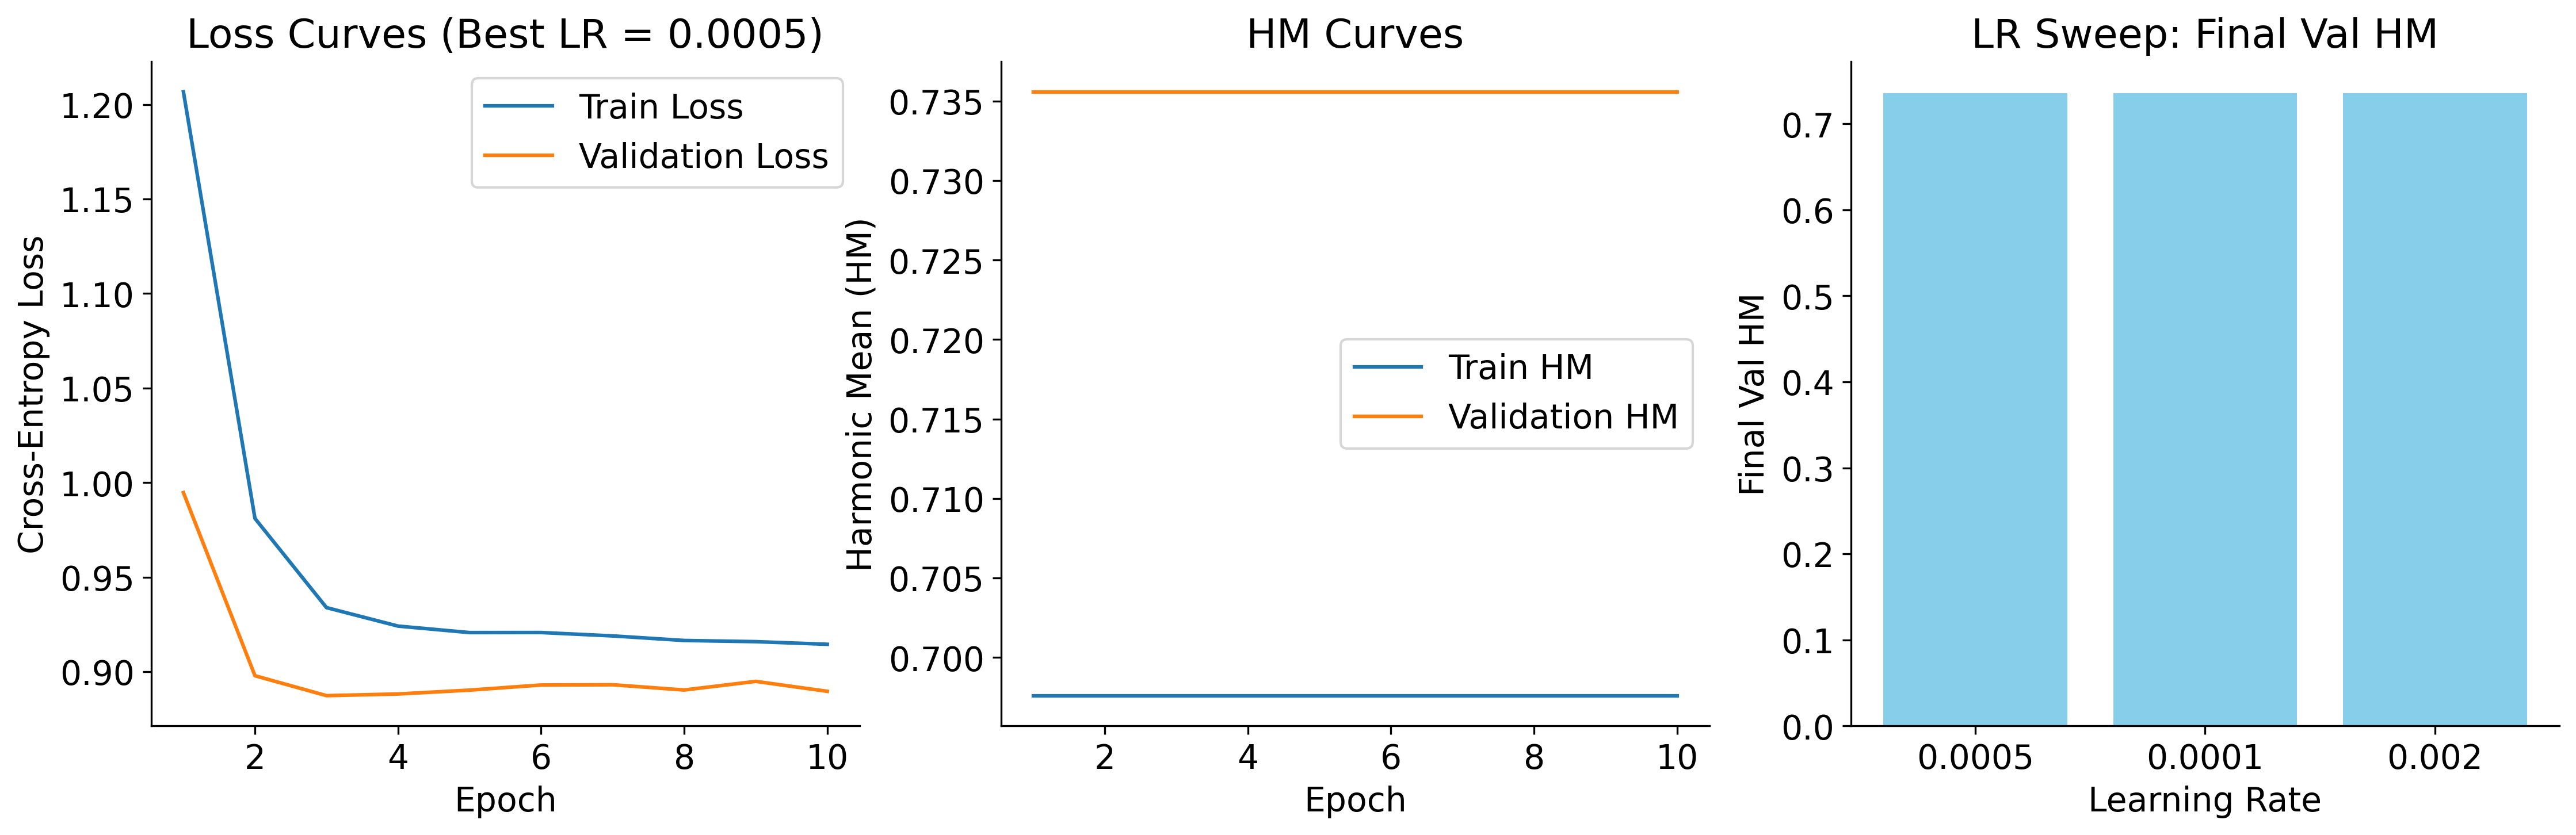
\includegraphics[width=0.9\linewidth]{baseline_overview.png}
\caption{Training accuracy with small vs.\ large batch sizes on a standard CNN. Large-batch models show erratic convergence and plateau early.}
\label{fig:baseline}
\end{figure}

\begin{figure}[t]
\centering
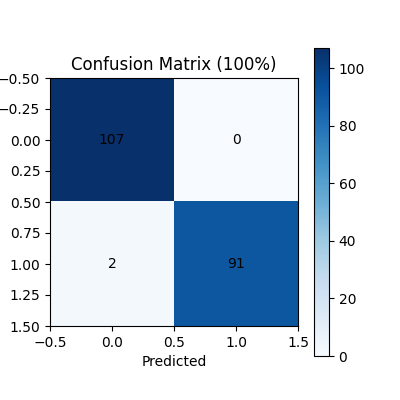
\includegraphics[width=0.9\linewidth]{confusion_matrix.png}
\caption{Confusion matrices comparing small-batch (left) and large-batch (right) regimes. Notice the increase in misclassified samples under large-batch training.}
\label{fig:confusion}
\end{figure}

\section{Conclusion}
We highlight that scaling batch sizes for image classification yields instability even in seemingly simple tasks. These observations caution practitioners against assuming linear speedups from large-batch methods. Future work includes studying specialized optimizers or adaptive regularization to offset batch-related gradient dynamics. We hope our negative results spark further discussion, helping the community mitigate large-batch pitfalls.

\appendix
\section{Additional Ablation Experiments}
We ablate model architectures (ResNet, simpler CNNs), initialization strategies, and scheduling adjustments. Figure~\ref{fig:ablation} displays that while small changes occasionally improve training stability, large-batch performance lags behind smaller-batch baselines in most scenarios.

\begin{figure}[h]
\centering
\includegraphics[width=0.65\linewidth]{ablation_analysis.png}
\caption{Additional ablation results. Each sub-figure corresponds to a distinct CNN variant with various training hyperparameters.}
\label{fig:ablation}
\end{figure}

\bibliographystyle{iclr2025_conference}
\bibliography{references}
\end{document}